% ===================== 0. Opening =====================
% Slide 2 -- the question, and a preview of the answer (revisited on the headline slide)

\begin{frame}{The question of this thesis}
  \begin{columns}[c]
    \begin{column}{0.42\textwidth}
      \begin{itemize}
        \item In a transversely polarized proton, unpolarized quarks are pushed \textbf{sideways}: the \textbf{Sivers effect}.
        \item Lattice QCD has computed the size of this push, but only \textbf{integrated over the momentum fraction $x$}.
        \item[]
        \item \textbf{Question:} can lattice QCD give the Sivers shift \textbf{as a function of $x$}?
      \end{itemize}
      \vspace{3mm}
      \keymsg{Where we are going: the Sivers shift as a function of $x$}
    \end{column}
    \begin{column}{0.56\textwidth}
      \centering
      \begin{tikzpicture}
        \node[opacity=0.35, inner sep=0pt] (img) {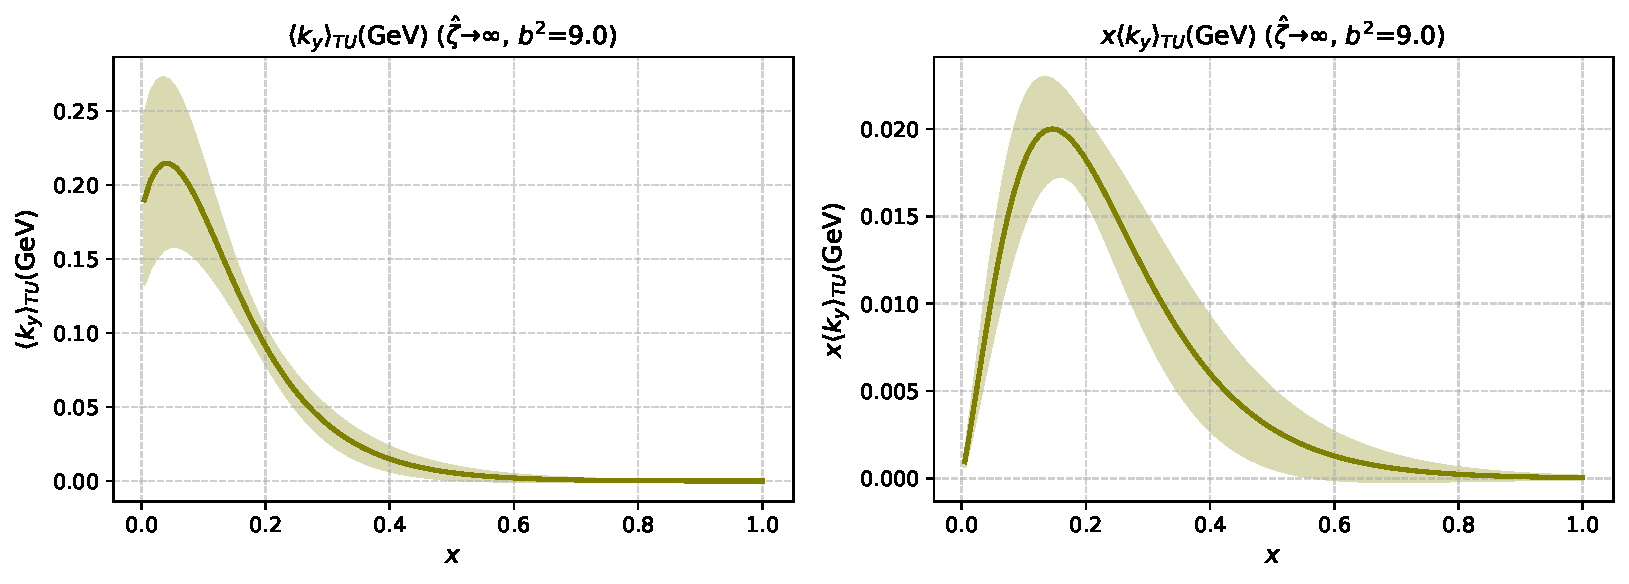
\includegraphics[width=\linewidth]{Extrapolated_AmpLevel_P234_Sivers_1_over_zetahat_sq_bmin3_eta610_b29.0_Sivers.pdf}};
        \node[draw=gray, fill=white, rounded corners, font=\large, anchor=south] at ([yshift=2mm]img.north) {\textbf{?}\ \ answer at the end};
      \end{tikzpicture}
    \end{column}
  \end{columns}
\end{frame}
